
\documentclass[11pt]{article}
\usepackage[a4paper,margin=1in]{geometry}
\usepackage[T1]{fontenc}
\usepackage[utf8]{inputenc}
\usepackage{lmodern,microtype}
\usepackage{amsmath,amssymb,amsthm,mathtools,bm}
\usepackage{graphicx,booktabs,float,enumitem}
\usepackage{xcolor}
\usepackage[colorlinks=true,linkcolor=blue!55!black,citecolor=blue!55!black,urlcolor=blue!55!black]{hyperref}
\usepackage[nameinlink,capitalise,noabbrev]{cleveref}

\newtheorem{theorem}{Theorem}[section]
\newtheorem{proposition}[theorem]{Proposition}
\newtheorem{corollary}[theorem]{Corollary}
\theoremstyle{definition}
\newtheorem{definition}[theorem]{Definition}
\newtheorem{remark}[theorem]{Remark}
\newtheorem{example}[theorem]{Example}

\newcommand{\C}{\mathbb C}
\newcommand{\D}{\mathrm D}
\newcommand{\Q}{\mathcal Q}
\newcommand{\B}{\mathcal B}
\newcommand{\Oterm}{\mathcal O}
\newcommand{\norm}[1]{\left\lVert #1\right\rVert}

\title{Tensorial Multidimensional Pandrosion\\
\large Averaged Jacobian Divided Differences, Bilinear Residual Laws, and Tensor-Flat Charts}
\author{Ivan Besevic\\Independent Mathematical Research\\\texttt{github.com/ivan-fr/poussiere\_de\_x}}
\date{May 2026}

\begin{document}
\maketitle

\begin{abstract}
The scalar anchored Pandrosion map replaces the monomial denominator by an anchored divided difference and makes a root into a fixed point whose multiplier is read from a secant slope. This paper develops the corresponding local theory for analytic systems $F:\C^n\to\C^n$. The scalar divided difference is replaced by the averaged Jacobian
\[
\Q_F(a,s)=\int_0^1 \D F(s+t(a-s))\,dt,
\qquad
F(a)-F(s)=\Q_F(a,s)(a-s),
\]
and the multidimensional anchored map is
\[
P_{F,a}(s)=a-\Q_F(a,s)^{-1}F(a).
\]
At a simple zero $r$, with $A=\D F(r)$ and $B=\D^2F(r)$, the local two-point law is
\[
P_{F,a}(s)-r=\frac12 A^{-1}B[a-r,s-r]+\Oterm\big((\|a-r\|+\|s-r\|)^3\big).
\]
Thus the raw fixed-anchor map has a linear multiplier controlled by the anchor vector through the bilinear tensor $A^{-1}B$. Under a chart $\phi$, the tensor $D^2(G\circ\phi)(0)$ is the multidimensional analogue of scalar curvature. A root-normalized chart is first-order tensor-flat precisely when
\[
D^2(G\circ\phi)(0)=0.
\]
The quadratic jet realizing this cancellation is the second-order local inverse jet of $G$. More generally, an $m$-flat chart satisfying $G(\phi(u))=u+\Oterm(\|u\|^{m+1})$ makes the local multiplier $\Oterm(\|a\|^m)$. Numerical figures for a two-dimensional analytic system illustrate the multiplier ladder, the anisotropy of anchor directions, and the enlarged low-error region produced by tensor cancellation.
\end{abstract}

\paragraph{One-sentence summary.}
Multidimensional Pandrosion replaces scalar slopes by averaged Jacobians; its first residual tensor is $\frac12 A^{-1}D^2F(r)$, and tensor-flat charts cancel that tensor before iteration begins.

\section{Introduction}

The scalar theory of anchored divided differences shows that a fixed anchor turns a simple zero into a fixed point and that the residual multiplier is the mismatch between a tangent slope and an anchor-root secant slope. The general analytic paper proves the scalar local product law
\[
P_{F,a}(s)-r \sim \frac{F''(r)}{2F'(r)}(a-r)(s-r),
\]
while the optimal-chart and higher-order papers show that one can reduce this residual factor by flattening the transformed equation in a suitable coordinate.

The purpose of the present paper is to move the same idea to systems. The correct object is not a scalar denominator but a matrix-valued divided difference. For a system $F:\C^n\to\C^n$, the natural average along the segment from $s$ to $a$ is
\[
\Q_F(a,s)=\int_0^1 \D F(s+t(a-s))\,dt.
\]
This operator satisfies the exact identity
\[
F(a)-F(s)=\Q_F(a,s)(a-s),
\]
which is the multidimensional replacement for the scalar divided difference.

The key observation is that the first residual obstruction is tensorial. If $r$ is a simple zero, $A=\D F(r)$, and $B=\D^2F(r)$, then
\[
P_{F,a}(s)-r=\frac12 A^{-1}B[a-r,s-r]+\text{higher order}.
\]
This formula is the multivariate version of the scalar fixed-anchor secant product law. It is also the formula behind the practical finite-slope engines: good anchors and well-conditioned averaged Jacobians are the natural geometric data.

\paragraph{Main contributions.}
The paper proves the following local facts.
\begin{enumerate}[label=(\roman*)]
\item The averaged-Jacobian map has exactly the same fixed-point property as the scalar anchored map.
\item The leading error is the bilinear tensor $\frac12 A^{-1}\D^2F(r)[a-r,s-r]$.
\item In a chart $\phi$, first-order tensor cancellation is the coordinate condition
\[
D^2(G\circ\phi)(0)=0.
\]
\item The unique quadratic jet satisfying this condition is the second-order inverse jet
\[
\phi_2(u)=\rho+A^{-1}u-\frac12 A^{-1}B[A^{-1}u,A^{-1}u].
\]
\item Higher-order inverse jets yield a tensorial $m$-flat hierarchy
\[
G(\phi_m(u))=u+\Oterm(\|u\|^{m+1})
\quad\Longrightarrow\quad
\|DP_{\phi_m,a}(0)\|=\Oterm(\|a\|^m).
\]
\end{enumerate}

\section{Averaged Jacobian divided differences}

Let $U\subset\C^n$ be a convex neighborhood and let $F:U\to\C^n$ be analytic.

\begin{definition}[Averaged Jacobian divided difference]
For $a,s\in U$, define
\begin{equation}\label{eq:Q}
\Q_F(a,s)=\int_0^1 \D F(s+t(a-s))\,dt.
\end{equation}
\end{definition}

By the fundamental theorem of calculus,
\begin{equation}\label{eq:exact-diff}
F(a)-F(s)=\Q_F(a,s)(a-s).
\end{equation}
Thus $\Q_F(a,s)$ is a canonical matrix-valued divided difference along the segment from $s$ to $a$.

\begin{definition}[Multidimensional anchored Pandrosion]
Assume $F(a)\neq0$ and $\Q_F(a,s)$ is invertible. The anchored multidimensional Pandrosion map is
\begin{equation}\label{eq:Pmulti}
P_{F,a}(s)=a-\Q_F(a,s)^{-1}F(a).
\end{equation}
Equivalently, using \eqref{eq:exact-diff},
\begin{equation}\label{eq:secant-form}
P_{F,a}(s)=s-\Q_F(a,s)^{-1}F(s).
\end{equation}
\end{definition}

\begin{proposition}[Fixed points]\label{prop:fixed}
Let $r$ be a zero of $F$, $F(a)\neq0$, and $\Q_F(a,r)$ be invertible. Then
\[
P_{F,a}(r)=r.
\]
Conversely, if $P_{F,a}(s)=s$ and $\Q_F(a,s)$ is invertible, then $F(s)=0$.
\end{proposition}

\begin{proof}
If $F(r)=0$, then \eqref{eq:exact-diff} gives $F(a)=\Q_F(a,r)(a-r)$, hence
\[
P_{F,a}(r)=a-\Q_F(a,r)^{-1}\Q_F(a,r)(a-r)=r.
\]
Conversely, $P_{F,a}(s)=s$ gives $\Q_F(a,s)(a-s)=F(a)$. By \eqref{eq:exact-diff}, the left side is $F(a)-F(s)$, so $F(s)=0$.
\end{proof}

\section{The tensor product law}

Let $r$ be a simple zero, and translate coordinates so $r=0$. Write
\[
F(w)=Aw+\frac12 B[w,w]+\frac16 C[w,w,w]+\Oterm(\|w\|^4),
\]
where $A=\D F(0)$ is invertible and $B=\D^2F(0)$ is a symmetric vector-valued bilinear map.

\begin{theorem}[Bilinear local residual law]\label{thm:bilinear}
Let $a=\alpha$ and $s=\sigma$ be close to $0$. Then
\begin{equation}\label{eq:bilinear-law}
P_{F,a}(s)
=
\frac12 A^{-1}B[\alpha,\sigma]
+
\Oterm\big(\|\alpha\|^2\|\sigma\|+\|\alpha\|\|\sigma\|^2+\|\sigma\|^3\big).
\end{equation}
Consequently the derivative of the fixed-anchor map at the root is
\begin{equation}\label{eq:multimult}
DP_{F,a}(0)v
=
\frac12 A^{-1}B[a,v]
+
\Oterm(\|a\|^2\|v\|).
\end{equation}
\end{theorem}

\begin{proof}
From the integral definition,
\[
\Q_F(\alpha,\sigma)v
=
Av+\frac12 B[\alpha+\sigma,v]
+\Oterm((\|\alpha\|^2+\|\alpha\|\|\sigma\|+\|\sigma\|^2)\|v\|).
\]
Therefore
\[
\Q_F(\alpha,\sigma)^{-1}
=
A^{-1}
-\frac12 A^{-1}B[\alpha+\sigma,A^{-1}(\cdot)]
+\Oterm((\|\alpha\|+\|\sigma\|)^2).
\]
Using the secant form,
\[
P_{F,a}(s)=\sigma-\Q_F(\alpha,\sigma)^{-1}F(\sigma),
\]
and
\[
F(\sigma)=A\sigma+\frac12 B[\sigma,\sigma]+\Oterm(\|\sigma\|^3).
\]
Substitution yields
\[
\Q_F(\alpha,\sigma)^{-1}F(\sigma)
=
\sigma+\frac12 A^{-1}B[\sigma,\sigma]
-\frac12 A^{-1}B[\alpha+\sigma,\sigma]+\text{higher order}
=
\sigma-\frac12 A^{-1}B[\alpha,\sigma]+\text{higher order}.
\]
Subtracting from $\sigma$ gives \eqref{eq:bilinear-law}. Differentiating with respect to $\sigma$ gives \eqref{eq:multimult}.
\end{proof}

\begin{remark}
The scalar formula is recovered by taking $A=F'(0)$ and $B=F''(0)$. Then \eqref{eq:bilinear-law} becomes
\[
P_{F,a}(s)=\frac{F''(0)}{2F'(0)}as+\cdots.
\]
\end{remark}

\section{Tensor-flat charts}

Let $G:\Omega\to\C^n$ be analytic and let $\rho$ be a simple zero. Let $\phi$ be a local biholomorphic chart with $\phi(0)=\rho$, and set
\[
F_\phi(u)=G(\phi(u)).
\]

\begin{definition}[Root-normalized and tensor-flat chart]
A chart $\phi$ is root-normalized if
\[
D(G\circ\phi)(0)=I.
\]
It is first-order tensor-flat if, in addition,
\[
D^2(G\circ\phi)(0)=0.
\]
More generally, it is $m$-flat if
\[
G(\phi(u))=u+\Oterm(\|u\|^{m+1}).
\]
\end{definition}

\begin{theorem}[Quadratic tensor cancellation]\label{thm:tensor-flat}
Let $A=DG(\rho)$ and $B=D^2G(\rho)$. The quadratic chart jet
\begin{equation}\label{eq:phi2}
\phi_2(u)=\rho+A^{-1}u-\frac12 A^{-1}B[A^{-1}u,A^{-1}u]
\end{equation}
is root-normalized and first-order tensor-flat:
\[
G(\phi_2(u))=u+\Oterm(\|u\|^3).
\]
It is the unique quadratic jet with these properties.
\end{theorem}

\begin{proof}
Write $\phi(u)=\rho+Lu+\frac12 H[u,u]+\Oterm(\|u\|^3)$. Root normalization forces $AL=I$, so $L=A^{-1}$. The quadratic term of $G\circ\phi$ is
\[
\frac12 AH[u,u]+\frac12 B[Lu,Lu].
\]
Setting it equal to zero gives
\[
H[u,u]=-A^{-1}B[A^{-1}u,A^{-1}u],
\]
which is exactly \eqref{eq:phi2}. Uniqueness follows because $A$ is invertible.
\end{proof}

\begin{corollary}[Tensor-flat multiplier order]
If $\phi$ is first-order tensor-flat, then
\[
\|DP_{\phi,a}(0)\|=\Oterm(\|a\|^2).
\]
If $\phi$ is $m$-flat, then
\[
\|DP_{\phi,a}(0)\|=\Oterm(\|a\|^m).
\]
\end{corollary}

\begin{proof}
Apply \cref{thm:bilinear} to $F_\phi=G\circ\phi$. If $D^2F_\phi(0)=0$, the bilinear tensor vanishes and the next term is quadratic in the anchor. The $m$-flat statement follows by the same Taylor expansion degree by degree.
\end{proof}

\section{Figures: a two-dimensional test system}

Consider
\[
G_1(x,y)=x+0.55x^2+0.25xy-0.15y^2,
\]
\[
G_2(x,y)=y-0.20x^2+0.35xy+0.50y^2.
\]
The root is $0$ and $DG(0)=I$. The tensor-flat quadratic chart is therefore
\[
\phi_2(u)=u-Q_2(u),
\]
where $Q_2$ is the quadratic part of $G$.

\begin{figure}[H]
\centering
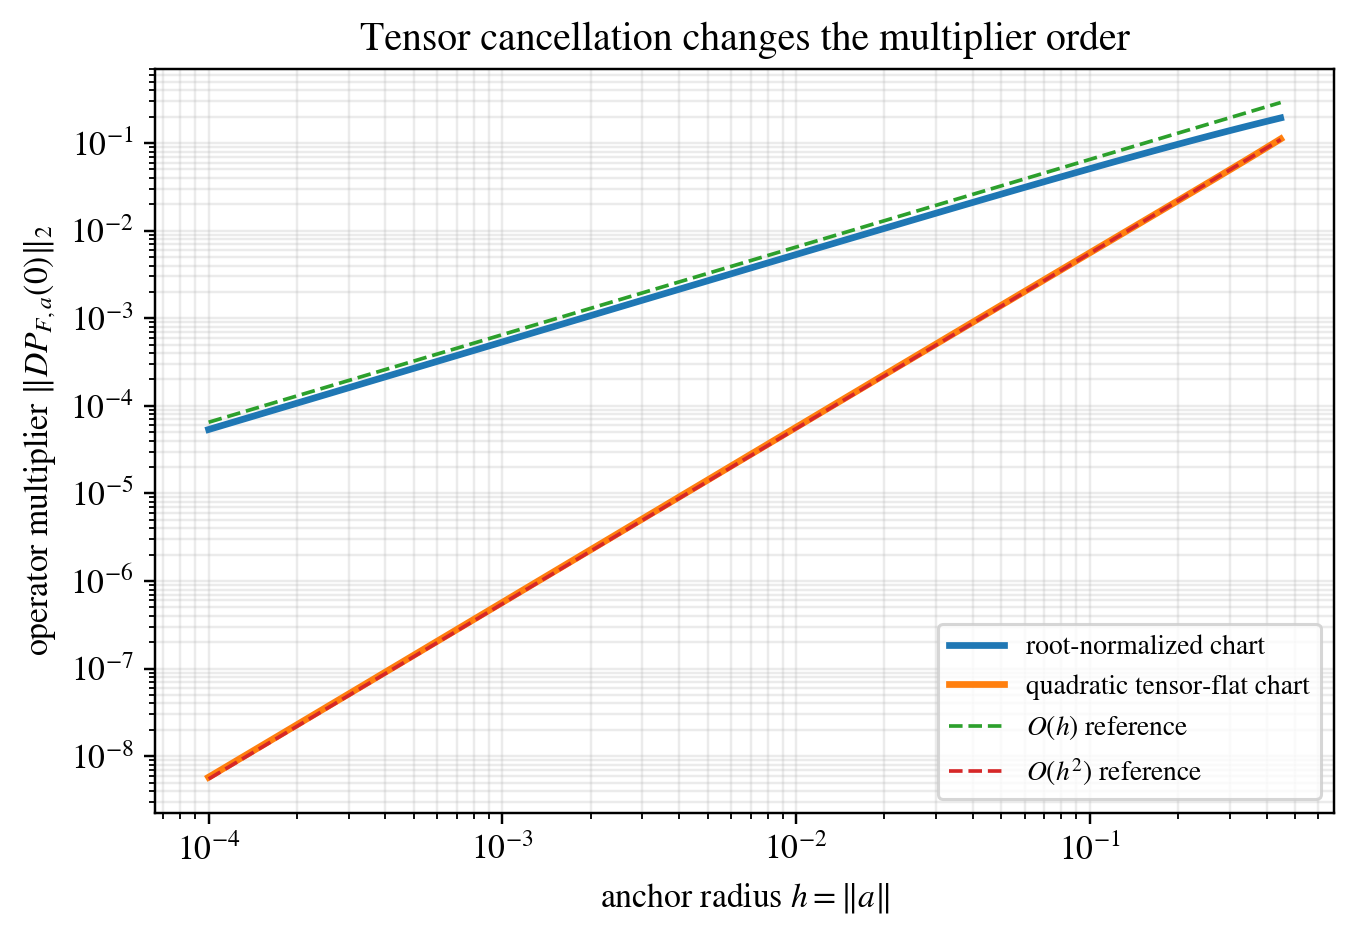
\includegraphics[width=.78\textwidth]{figures/fig_tensor_multiplier_ladder.png}
\caption{Multiplier norm versus anchor radius. The root-normalized chart has slope $1$ on a log-log scale, while the tensor-flat chart has slope $2$, confirming the tensor cancellation law.}
\end{figure}

\begin{figure}[H]
\centering
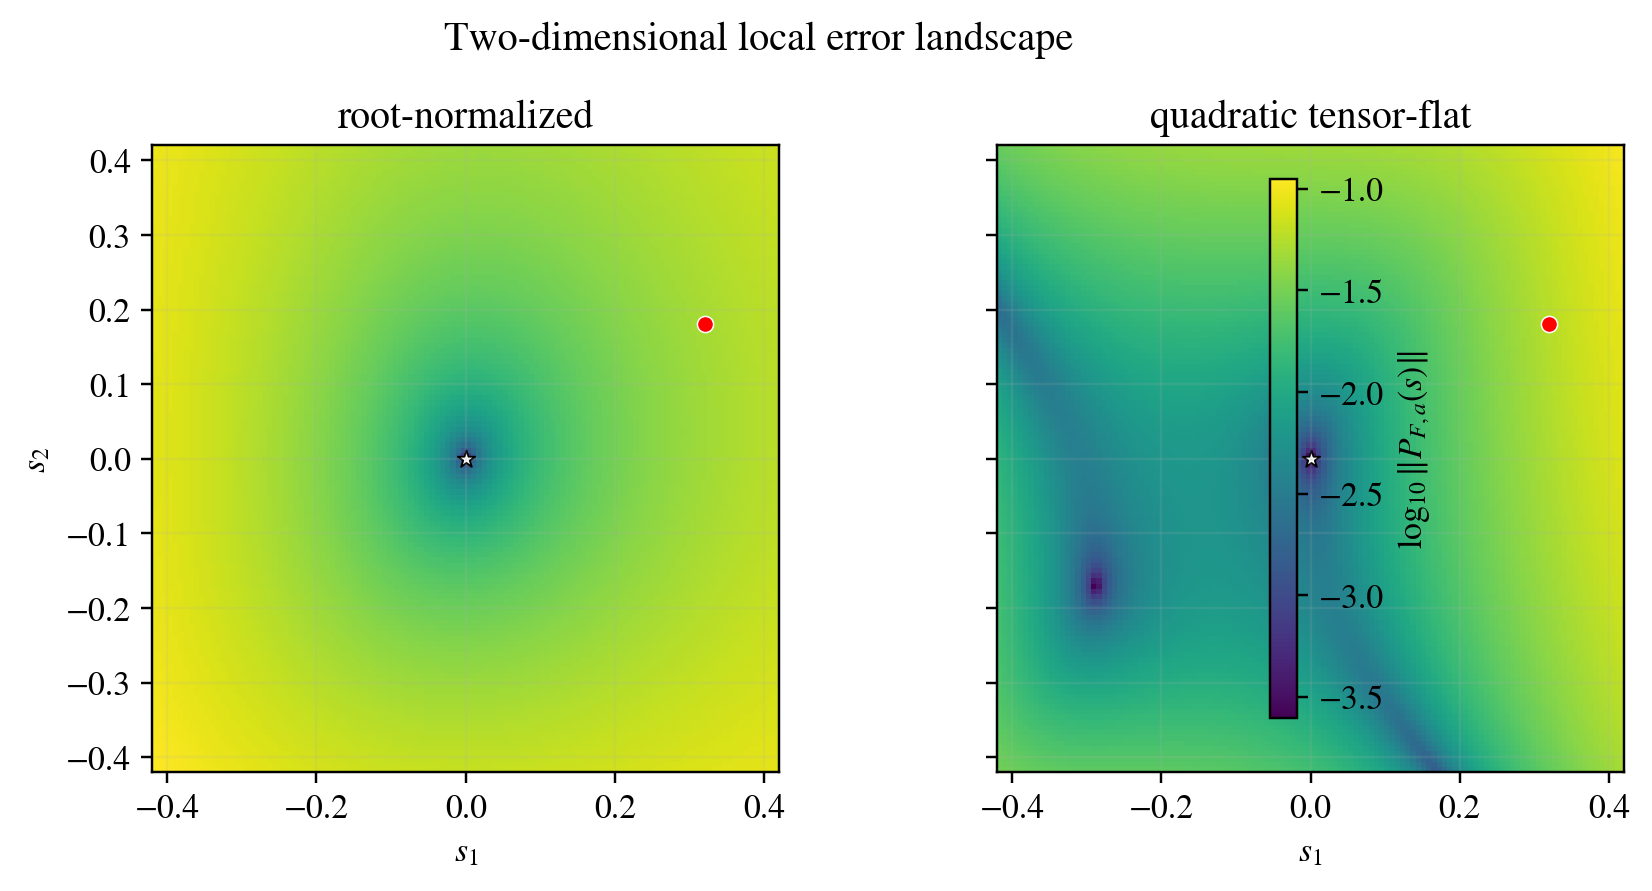
\includegraphics[width=.96\textwidth]{figures/fig_tensor_error_landscape.png}
\caption{Local error landscape for a fixed anchor. Darker regions correspond to smaller $\|P_{F,a}(s)\|$. Tensor cancellation enlarges the low-error region around the root.}
\end{figure}

\begin{figure}[H]
\centering
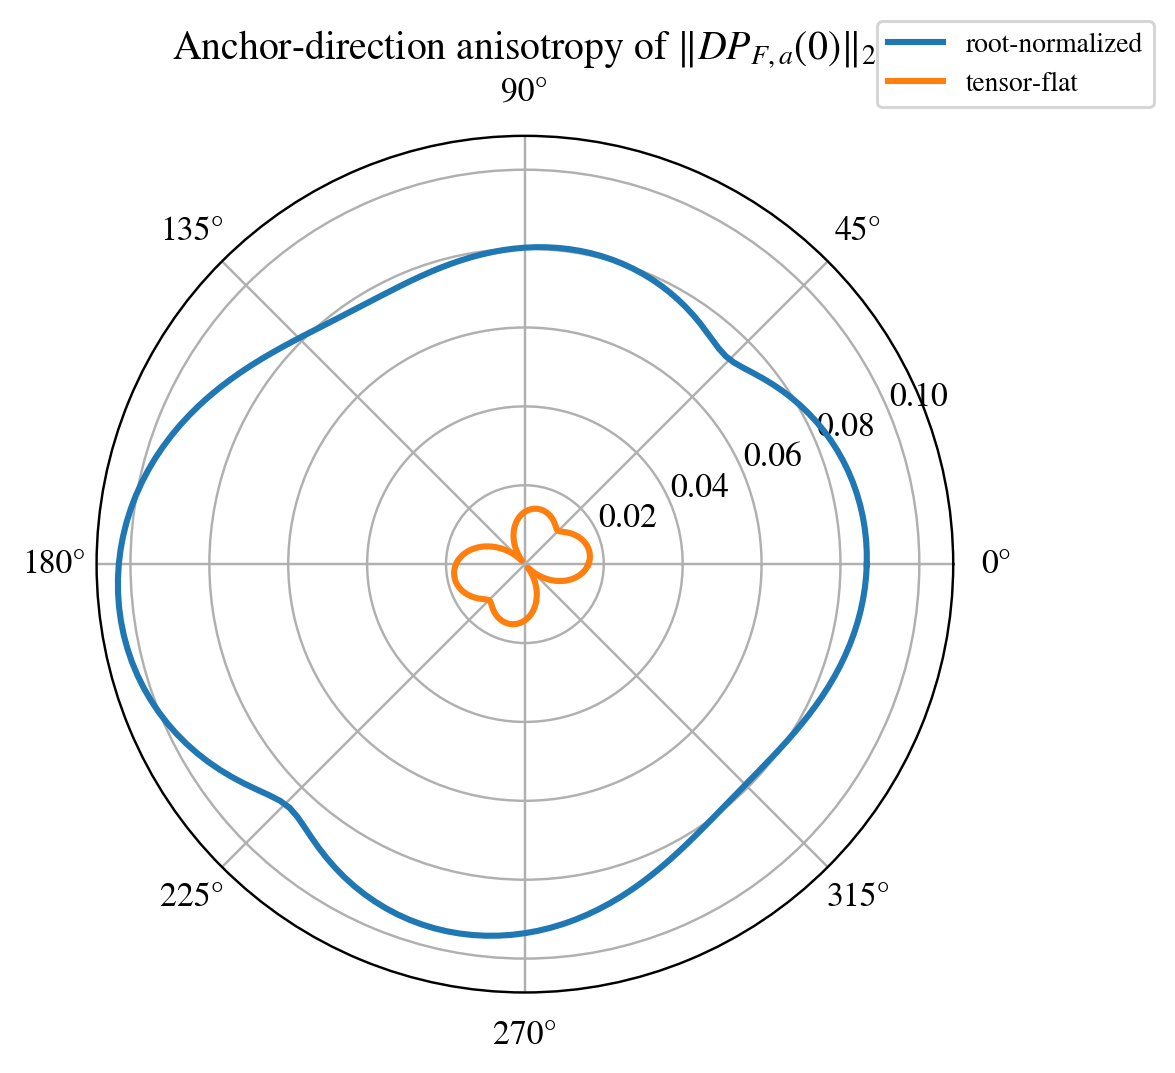
\includegraphics[width=.70\textwidth]{figures/fig_tensor_anisotropy.png}
\caption{The bilinear tensor $A^{-1}B[a,\cdot]/2$ makes the multiplier anisotropic in the anchor direction. Tensor-flat coordinates suppress the leading anisotropic lobe.}
\end{figure}

\section{Discussion}

The multidimensional theory clarifies what the finite-slope engines are approximating. They are not merely using random secants; they are sampling averaged Jacobians whose local defect is governed by a symmetric bilinear tensor. The practical lessons are direct:
\begin{enumerate}[label=(\arabic*)]
\item choose anchors that reduce $\|A^{-1}B[a,\cdot]\|$;
\item reject probes for which $\Q_F(a,s)$ is poorly conditioned;
\item use chart transformations to cancel the quadratic tensor when derivative information is available or estimable.
\end{enumerate}

This is the natural bridge between pure Pandrosion engines and higher-order geometric preconditioning. The scalar curvature condition becomes a tensor cancellation condition. Higher-order inverse jets become symmetric multilinear normal forms.

\section{Conclusion}

Multidimensional Pandrosion is governed by an averaged Jacobian divided difference. At a simple zero, the first nontrivial residual is the bilinear tensor
\[
\frac12 (DF(r))^{-1}D^2F(r)[a-r,s-r].
\]
A chart can cancel this tensor, and the quadratic inverse jet gives the unique local cancellation. This provides a clean tensorial continuation of the scalar anchored divided-difference program.

\begin{thebibliography}{9}
\bibitem{monomial}
I. Besevic, \emph{A Monomial Pandrosion Scheme: Contraction, Chart Scaling, and Steffensen Acceleration for $z^p=x$}, manuscript, May 2026.
\bibitem{general}
I. Besevic, \emph{Anchored Pandrosion for General Analytic Equations}, manuscript, May 2026.
\bibitem{charts}
I. Besevic, \emph{Optimal Geometric Charts for Anchored Divided-Difference Iterations}, manuscript, May 2026.
\bibitem{jets}
I. Besevic, \emph{Higher-Order Jet Cancellation for Anchored Divided-Difference Iterations}, manuscript, May 2026.
\bibitem{ortega}
J. M. Ortega and W. C. Rheinboldt, \emph{Iterative Solution of Nonlinear Equations in Several Variables}, Academic Press, 1970.
\bibitem{traub}
J. F. Traub, \emph{Iterative Methods for the Solution of Equations}, Prentice--Hall, 1964.
\end{thebibliography}

\end{document}
